\section{Kapacitetudnyttelse}
For at analysere OA's ressourcer ift. patientbyrden, benyttes udtrykket kapacitetsudnyttelse. Kapacitetudnyttelse betegner forholdet mellem aktivitet og kapacitet. Aktivitet omhandler patient og kontakt, herunder består kontakt af forundersøgelse, behandling og kontrol. Kapacitet omfatter antallet af personale, udstyr og rum, hvor personalet består af læger, sygeplejersker og sekretærer. Udstyret beskriver antallet af maskiner på en afdeling og antallet af rum beskriver opbevarelsen af udstyret. Den samlede kapacitetsudnyttelse er defineret ud fra, at der produceres mest muligt for de investerede ressourcer.\cite{Company2013} 

\begin{figure}[H]
	\flushleft 
	\centering
	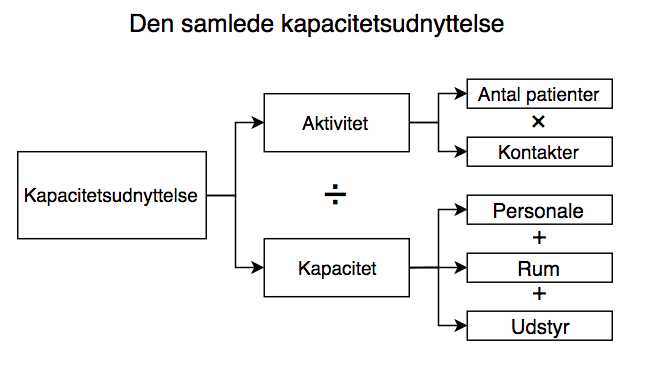
\includegraphics[scale=.5]{figures/Kapacitetsudnyttelse.png}
	\flushleft
	\caption{\textit{Den samlede kapacitetsudnyttelse, som er definineret ved forholdet mellem aktivitet og kapacitet. Aktivitet omfatter antallet af patienter samt kontakter og kapacitet omfatter personale, rum og udstyr.}\cite{Company2013}}
	\label{kapacitet}
\end{figure}

\noindent
Ud fra \figref{kapacitet} fremgår det, at kapacitetsudnyttelse er forholdet mellem aktivitet og kapacitet. Dertil ses aktivitet som antal patienter multipliceret med kontakter. Kapaciteten udgør personale, rum og udstyr sammenlagt. Antallet af patienter, der repræsenterer en del af aktivitet beskriver ligeledes belægning på hospitalets afdelinger.\cite{Company2013} 

Belægning er defineret ud fra antallet af patienter, der er normeret til på en afdeling\cite{Heidmann2014}. Når en $100~\%$ belægning opnås, svarer dette til, at de disponible sengepladser på en afdeling er taget i brug. Ved en belægning på over $100~\%$ betyder det, at der er flere patienter end afdelingen er normeret til, hvilket vil sige, at afdelingen yder mere end der er kapacitet til. Ud fra \figref{kapacitet} vil dette betyde, at der ikke er ligevægt mellem aktivitet og kapacitet, hvilket i dette tilfælde vil forårsage kapacitetsmangel, dvs. en belægningsgrad over $100~\%$, på afdelingen. 


\subsubsection{Belægningsgrad på ortopædkirurgisk afdeling}\label{omfang}
På OA opleves en varierende belægningsgrad for hver måned. Som tidligere nævnt ønskes en fuld kapacitetsudnyttelse, hvoraf alle sengepladser ønskes at være i brug. Belægningsgraden er antallet af de anvendte disponible senge. På \figref{maxminbelaeg} ses belægningsgraden fra år $2014$ til $2015$ på ortopædkirurgisk afdeling.\cite{SDS2015}

\begin{figure}[H]
	\flushleft 
	\centering
	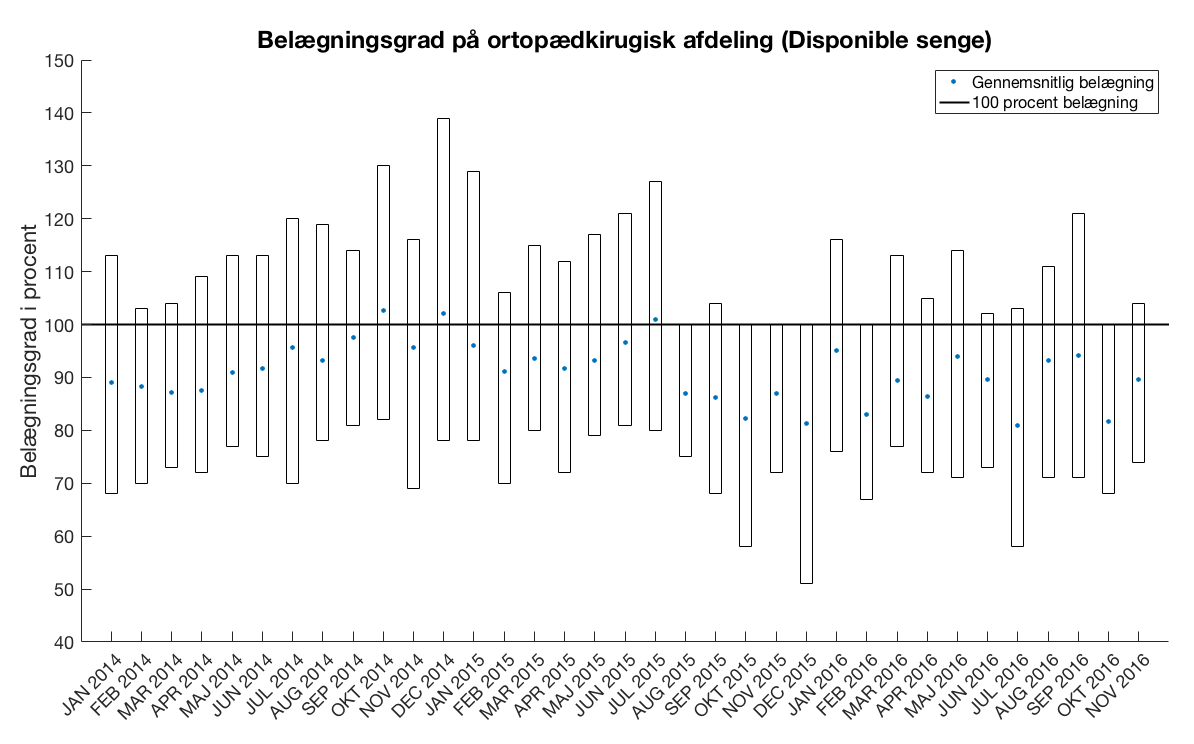
\includegraphics[scale=.45]{figures/belaegningsgradny.png}
	\flushleft
	\caption{\textit{Belægningsgraden på OA målt over $35$ måneder fra år $2014$ til $2016$. Søjlerne viser belægning ift. $100~\%$, hvortil maksimal og minimum belægning ligeledes illustreres. De blå punkter viser den gennemsnitlige belægning for hver måned.}\cite{SDS2015}}
	\label{maxminbelaeg}
\end{figure}

\noindent
Det fremgår af \figref{maxminbelaeg}, at OA oplever en belægning hhv. over og under den ønskede belægning på $100~\%$. Den maksimale belægning fremkommer i december måned år 2014 og er på $139~\%$. Maksimums belægning kan indikere, at der er flere indlagte patienter end afdelingen er disponeret til, herved har afdelingen oplevet kapacitetsmangel. Minimums belægning forekommer i december måned år 2015 og er på $51~\%$. Dette kan indikere, at der ikke har været tilstrækkelige elektive patienter i perioder, hvilket ligeledes medfører ubalance i kapacitetsudnyttelsen. Af \figref{maxminbelaeg} er den gennemsnitlige belægning pr. måned hyppigst under $100~\%$. I oktober samt december måned år $2014$ og juli år 2015 opleves dog en gennemsnitlig belægning over $100~\%$. Den gennemsnitlige belægning ses varierende mellem $80$ og $100~\%$ for de resterende måneder, hvilket kan indikere, at afdelingen oplever kapacitetsmangel i kortvarige perioder.\cite{SDS2015} 
Det fremgår ikke af den anvendte data, hvorvidt belægningen over $100~\%$ opleves i timer eller flere døgn. Dertil skal der tages forbehold for, at det ikke er angivet, hvorvidt det er elektive eller akutte patienter, der udgør en belægning over $100~\%$.\cite{SDS2015} 
For at underbygge belægningsgraden yderligere, illustrerer \figref{andeldage} andel af dage med en belægningsgrad på over $100~\%$ pr. måned. 

Denne graf er udarbejdet ud fra OA over de samme 35 måneder som \figref{maxminbelaeg}.\cite{SDS2015} 

\begin{figure}[H]
	\flushleft 
	\centering
	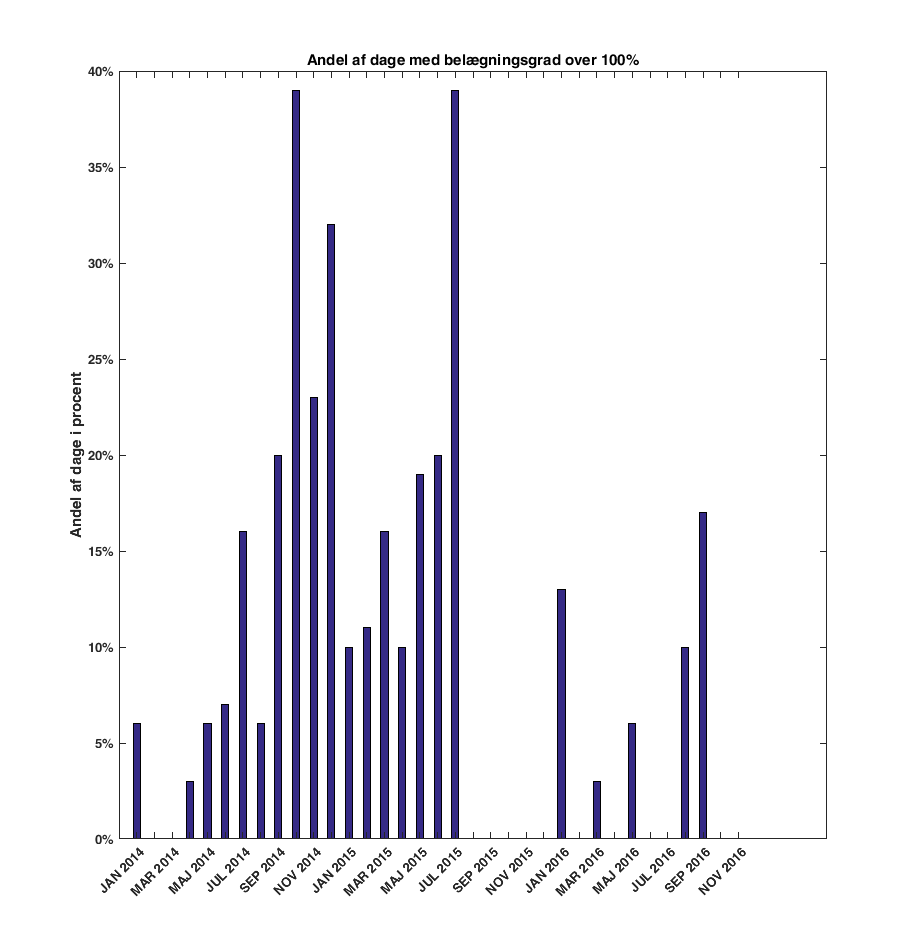
\includegraphics[scale=.4]{figures/andelAfDage.png}
	\flushleft
	\caption{\textit{Andel af dage med en belægning over $100~\%$ for OA målt over $35$ måneder fra år $2014$ til $2016$.}\cite{SDS2015}}
	\label{andeldage}
\end{figure}

\noindent
Det fremgår af \figref{andeldage}, at der i oktober måned år $2014$ samt juli måned år 2015 opleves en belægning på over $100~\%$ i $39\%$ af måneden. Sammenlignes der med \figref{maxminbelaeg} ses der i oktober måned år 2014 en belægning på $130~\%$. Juli måned år 2015, der ligeledes havde en belægning over $100\%$ i $39\%$ af måneden, oplevede en belægning på $127\%$. 
Ud fra den anvendte data fremgår det ikke, hvor mange patienter, der udgør en belægningsgrad over $100~\%$, samt hvor længe de enkelte patienter er indlagt på afdelingen. Da belægningsgraden og andel af dage med belægningsgrad over $100~\%$ kan variere for hver måned, anses $35$ måneder ikke som værende repræsentativ for at kunne vurdere problemets omfang. Ud fra belægningsgraden kan det dog tyde på, at en effektivisering af planlægningen af patienter på OA vil kunne medføre en balance i kapacitetsudnyttelsen.
